\begin{figure}[htbp]
\centering
\caption{Predictors of Late-Pretreatment Bilateral Connectivity}
\label{fig:bilateral_coefplot_pretreat}

\begin{threeparttable}

\begin{subfigure}{\textwidth}
    \centering
    \caption{Panel A: Proximity Measures}
    \label{fig:bilateral_coefplot_pretreat_proximity}
    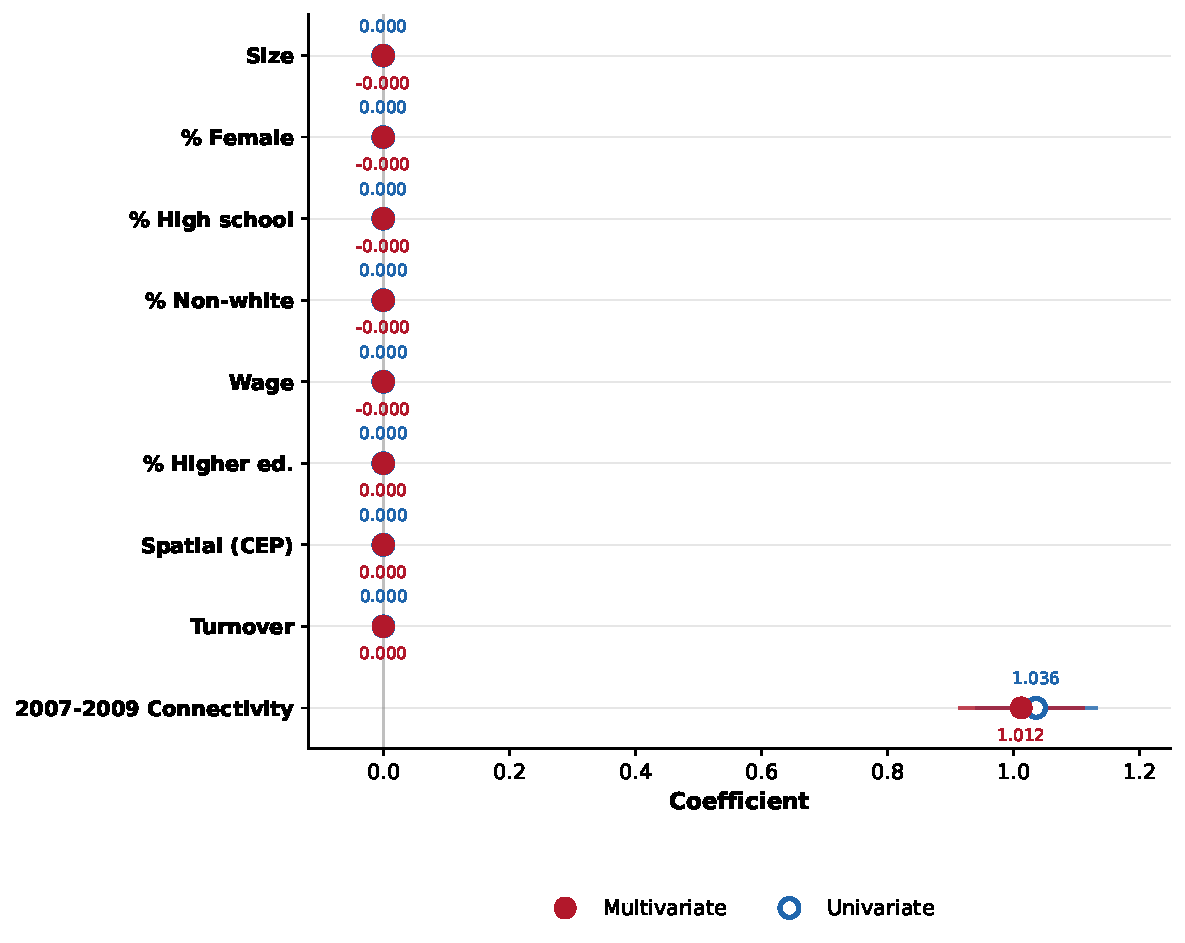
\includegraphics[width=0.85\textwidth]{coefplot_bilateral_pretreat_proximity.pdf}
\end{subfigure}

\vspace{1em}

\begin{subfigure}{\textwidth}
    \centering
    \caption{Panel B: Categorical Indicators}
    \label{fig:bilateral_coefplot_pretreat_dummies}
    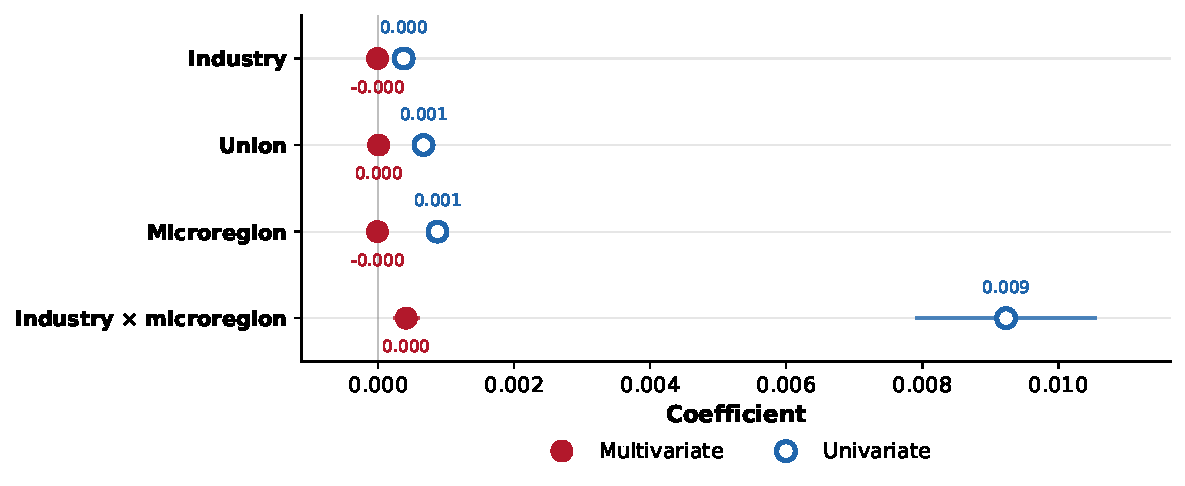
\includegraphics[width=0.85\textwidth]{coefplot_bilateral_pretreat_dummies.pdf}
\end{subfigure}

\begin{tablenotes}
\footnotesize
\item \textit{Notes:} This figure shows coefficients from regressions of late-pretreatment bilateral connectivity (2009--2011, based on year pairs 2009--10 and 2010--11) on establishment pair characteristics. Hollow blue markers show univariate regressions (each predictor separately); filled red markers show multivariate regressions (all predictors simultaneously, including early-pretreatment connectivity 2007--2009). All regressions control for establishment $i$ fixed effects. Bilateral connectivity is measured as the person-weighted average flow of workers between establishment pairs. Proximity measures are defined as the negative absolute difference between establishment characteristics (standardized), so higher values indicate greater similarity. Spatial proximity is measured as the negative log of distance between establishment postal code (CEP) centroids. Turnover proximity is measured as the negative absolute difference in establishment turnover rates. CBA clauses proximity is based on the number of clauses in collective bargaining agreements. Same-category dummies equal one if both establishments share the indicated category. Establishment characteristics are based on 2009--2011 averages. Horizontal lines represent 95\% confidence intervals based on robust standard errors. All regressions include the universe of establishment pairs, including those with zero worker flows.
\end{tablenotes}

\end{threeparttable}
\end{figure}
